\documentclass{article}
\usepackage[margin=0.5in]{geometry}
\usepackage[utf8]{inputenc}
\usepackage{graphicx}
\usepackage{hyperref}
\usepackage{color}
\usepackage{amsmath,amssymb}
\usepackage{algorithm}
\usepackage{algorithmic}

\title{UMass CMPSCI 383 (AI) HW2: Chapters 4-6}
\author{\textbf{Tony Gao}}
\date{Assigned: Sep 21 2017; Due: Oct 3 2017 @ 11:55 PM EST}

\begin{document}

\maketitle

\begin{abstract}
    Submit a (.zip) file to Moodle containing your latex (.tex) file, rendered pdf, and code. All written HW responses should be done in latex (use sharelatex.com or overleaf.com). All code should be written in Python and should run on the edlab machines ([yourusername]@elnux[1,2,...].cs.umass.edu).
\end{abstract}

\section{Gradient Descent}
Recall that gradient ascent is a form of hill-climbing to find maxima of a function using the update $\vec{x}_{k+1} \leftarrow \vec{x}_k + \alpha \nabla f (\vec{x}_k)$ with $\alpha > 0$. Note that $\vec{x}$ is a vector of real numbers, ie., $\vec{x} = [x_1,\ldots,x_n]$. Here, we will use gradient descent to find minima of a function using a similar update:
\begin{align}
\vec{x}_{k+1} \leftarrow \vec{x}_k - \alpha \nabla f (\vec{x}_k),
\end{align}
where $\vec{x}_k$ is gradient descent's $k$-th guess at the vector that minimizes $f(\vec{x})$.

\subsection{Bottom of a Bowl}
As a warm up, consider minimizing the function, $f(\vec{x}) = x_1^2 + x_2^2$. This function can be written succinctly as $f(\vec{x}) = ||\vec{x}||^2$ and is known as the $L_2$-norm of $\vec{x}$. It appears often in machine learning problems. The global minimum of this function is at the origin, $\vec{x}=[0,0]$.

(5 pts) Starting with $\vec{x}_0 = [2,-1]$, and $\alpha = 0.1$, report the first 3 steps of gradient descent. Does the function appear to be approaching the global minimum at the origin? If not, what's the problem and what's causing it?\\

The function appears to approach the global minimum. Each step brings the result closer to [0,0] and it is clear that subsequent steps will approach [0,0].

% The ampersand's (&) control where the 3 equations are aligned.
\begin{align}
    x_1 &= \textbf{[2,-1] - .1[4,-2] } &= [1.6, -.8]  \\
    x_2 &= \textbf{[1.6, -.8] - .1[3.2, -1.6]} &= [1.28, -.64] \\
    x_3 &= \textbf{[1.28, -.64] - .1[2.56,-1.28]} &= [1.024, -.512]
\end{align}

(5 pts) Starting with $\vec{x}_0 = [2,-1]$, and $\alpha = 1.5$, report the first 3 steps of gradient descent. Does the function appear to be approaching the global minimum at the origin? If not, what's the problem and what's causing it?\\

The function does not appear to be approaching the global minimum. The choice of $\alpha$ is causing the descent function to oscillate away from the origin. 

\begin{align}
    x_1 &= \textbf{[2,-1] - 1.5[4,-2]} &= [-4,2] \\
    x_2 &= \textbf{[-4,2] - 1.5[-8,4]} &= [8,-4] \\
    x_3 &= \textbf{[8,-4] - 1.5[16,-8]} &= [-16,8]
\end{align}

\subsection{Non-convex (messy) Function}
Now, consider minimizing the 1-d function, $f(x) = 2 + x^2 - 2 \cos(10x)$. Note that the argument to cosine is interpreted as radians, not degrees (e.g., $\cos(\pi/2) = 0)$. The global minimum of this function is at $x=0$. When you compute the updates, round $\frac{\partial f}{\partial x}$ to two decimal places. Also round each new $x_k$ to two decimal places after each iteration. In other words,

\begin{align}
    \vec{x}_{k+1} \leftarrow Round(\vec{x}_k - \alpha Round(\nabla f (\vec{x}_k),2),2).
\end{align}

(5 pts) Starting with $x_0 = 100$, and $\alpha = 0.1$, report the first 3 steps of gradient descent. Does the function appear to be approaching the global minimum at zero? If not, what's the problem and what's causing it? \\

The function appears to be approaching x=0

\begin{align}
    \frac{\partial f}{\partial x} &= \textbf{2x+20$\sin(10x)$}
\end{align}

\begin{align}
    x_1 &= \textbf{Round(100-.1(216.54),2)} &= 78.35 \\
    x_2 &= \textbf{Round(78.35-.1(137.76),2)} &= 64.57 \\
    x_3 &= \textbf{Round(64.57-.1(109.25),2)} &= 53.65
\end{align}

(5 pts) Starting with $x_0 = 10$, and $\alpha = 0.01$, report the first 3 steps of gradient descent. Does the function appear to be approaching the global minimum at zero? If not, what's the problem and what's causing it?\\

The function enters an infinite loop, it does not appear to be approaching 0. The value of $x_k$ always rounds to 9.90. The issue is the choice of $\alpha=.01$. With step size .01, the descent by the gradient is rounded away causing the infinite loop. If $\alpha=.1$ is used, the function appears to approach 0. 

\begin{align}
    x_1 &= \textbf{Round(10-.01(9.87),2)} &= 9.90 \\
    x_2 &= \textbf{Round(9.90 - .01(-0.18),2)} &= 9.90 \\
    x_3 &= \textbf{Round(9.90 - .01(-0.18),2)} &= 9.90
\end{align}

(5 pts) Starting with $x_0 = 2.3$, and $\alpha = 0.01$, report the first 3 steps of gradient descent. Does the function appear to be approaching the global minimum at zero? If not, what's the problem and what's causing it?\\

The function does not appear to be approaching 0. If $\alpha = .1$ is used, the function appears to approach 0. Four test iterations with this shows f approaching 0: $x_4$ = 2.3-.1(-12.32)-.1(11.95)-.1(-15.05)-.1(20.58) = 1.78

\begin{align}
    x_1 &= \textbf{Round(2.3-.01(-12.32),2)} &= 2.42 \\
    x_2 &= \textbf{Round(2.42-.01(-11.23),2} &= 2.53 \\
    x_3 &= \textbf{Round(2.53-.01(8.39),2)} &= 2.45 \\
\end{align}

\section{Constraint Satisfaction Problems}
Implement a constraint satisfaction solver for solving Sudoku puzzles. We have provided a \texttt{my\_hw1.py} template and a Sudoku class in \texttt{sudoku.py} with convenient methods (e.g, loading a Sudoku puzzle from a text file). We've given you 6 Sudoku puzzles to debug your code on. We will be testing your code on 10 held-out Sudoku puzzles. You will receive points for getting the correct solution as well as the correct number of guesses needed for your CSP solver to solve the held-out puzzles. Consider every time you check whether an assignment is consistent as a guess (see last slide on backtracking in Lecture 5-6). Partial credit may be given if you correctly solve the 6 puzzles we've given you, but your solver fails on the held-out puzzles.

\subsection{Binary Constraints} (10pts) Show that the number of binary constraints required to represent a Sudoku problem is 810 (Hint: recall that the numbers on each column and row must be distinct, as well as on each 3x3 square).\\

Each variable can be associated with 8 variables in its column, 8 variables in its row, and 8-4=4 in its box that have not already been accounted for in the col/row. There are 81 total variables. This gives 81 * 20 associations = 1620 associations. Of these associations, only half are distinct. Each association is counted twice. For example, the association A1 != A9 for cell A1 is also counted in A9 != A1 for A9. This gives 1620/2=810 distinct binary constraints.

\subsection{Backtracking} (20pts) Implement the backtracking algorithm described in Figure 6.5 of the textbook. Your CSP solver should return a list of lists representation of the solved Sudoku puzzle as well as the number of guesses (assignments) required to solve the problem. Please see the comments in the code for more details. In your backtracking search implementation, order the Sudoku tile variables by the order they would be read on a page (left to right, up to down) and order the domain values by ascending order. Include the number of guesses required for each of the 6 practice puzzles below. Also include a folder of your solved Sudoku puzzles as text files in your submission.\\
\\
\begin{center}
\begin{tabular}{c||c}
    puzzle & \# of guesses \\ \hline
    001 & 541 \\ \hline
    026 & 20079 \\ \hline
    051 & 104112 \\ \hline
    076 & 45179 \\ \hline
    090 & 46719 \\ \hline
    100 & 206891 \\ \hline
\end{tabular}
\end{center}



\subsection{Heuristics} (15pts) Augment the backtracking algorithm with the MRV (minimum-remaining-value) heuristic, and observe the resulting savings in terms of number of guesses compared to plain backtracking. Include the number of guesses required for each of the 6 practice puzzles below. Also include a folder of your solved Sudoku puzzles as text files in your submission.\\
\\
\begin{center}
\begin{tabular}{c||c}
    puzzle & \# of guesses \\ \hline
    001 & 41 \\ \hline
    026 & 125 \\ \hline
    051 & 179 \\ \hline
    076 & 146 \\ \hline
    090 & 110 \\ \hline
    100 & 142 \\ \hline
\end{tabular}
\end{center}

\section{Alpha-Beta Pruning} Consider the tic-tac-toe problem, where players take turns in placing O's or X's until one of the players has a three-in-a-row (or column or diagonal).

\subsection{State Representation} (5pts) Explain how symmetries in the placement of X's and O's on the tic-tac-toe board can be exploited to dramatically shrink the search tree. Draw the resulting search tree down to a depth of 2 given the start state and \texttt{TicTacToe-SearchTree-Template} provided at~\href{https://docs.google.com/drawings/d/1l1VsrFXYuovPLV1bjBi_lMqEekN98_nCWesdhMv0kmo/edit?usp=sharing}{\color{blue}{HWs Public/HW2}}; make a copy and move the copy to your own Google Drive to edit it. You will fill out the figure with minimax values in the next question.\\

There are 3 possible $X_1$ moves : the corner, the side, and the center. Any of these 3 moves has rotational/reflection symmetry such that the board can be translated to generate equivalent board states with $X_1$ placements in other locations that have the same set of actions and results, so only these three states need be considered for expansion. This also follows for subsequent placements of O and X, significantly reducing the size of the search tree. For example, it does not matter if $O_1$ is placed in the top right or bottom left corner if $X_1$ is placed in the top left corner, as both placements of $O_1$ can be rotated and reflected to yield the other, therefore only one of these need to be represented in the tree. \\

Additionally, given that X moves first, if $O_1$ is placed on an edge, then X is guaranteed to win by creating an unavoidable multiple possible win scenario, so any placement of $O_1$ on an edge is never optimal and can be pruned from the search tree. For the purposes of this problem I do not prune these moves, I assume they are to be left in the tree.

\subsection{Minimax with Evaluation Heuristic} (10pts) For tic-tac-toe, there are a little less than 9! (362,880) leaf nodes (possible endings of the game). This is too many to draw on a page, so let's consider using an evaluation function, Eval(node), down to a depth of 2. Eval(node) returns N(Player X) - N(Player O) where N(Player $i$) gives the number of complete rows, columns, and diagonals that are still open for player $i$. A depth of 2 is too shallow to observe a winning move, but for completeness, define Eval(node) to be +infinity when X wins, and -infinity when O wins. Compute the minimax values for each node in the tree you drew above using the evaluation function, Eval(node). Include the search tree with the minimax values here.\\
\\
See Figure~\ref{fig:minimax_tree}.
\begin{figure}[h]
    \centering
    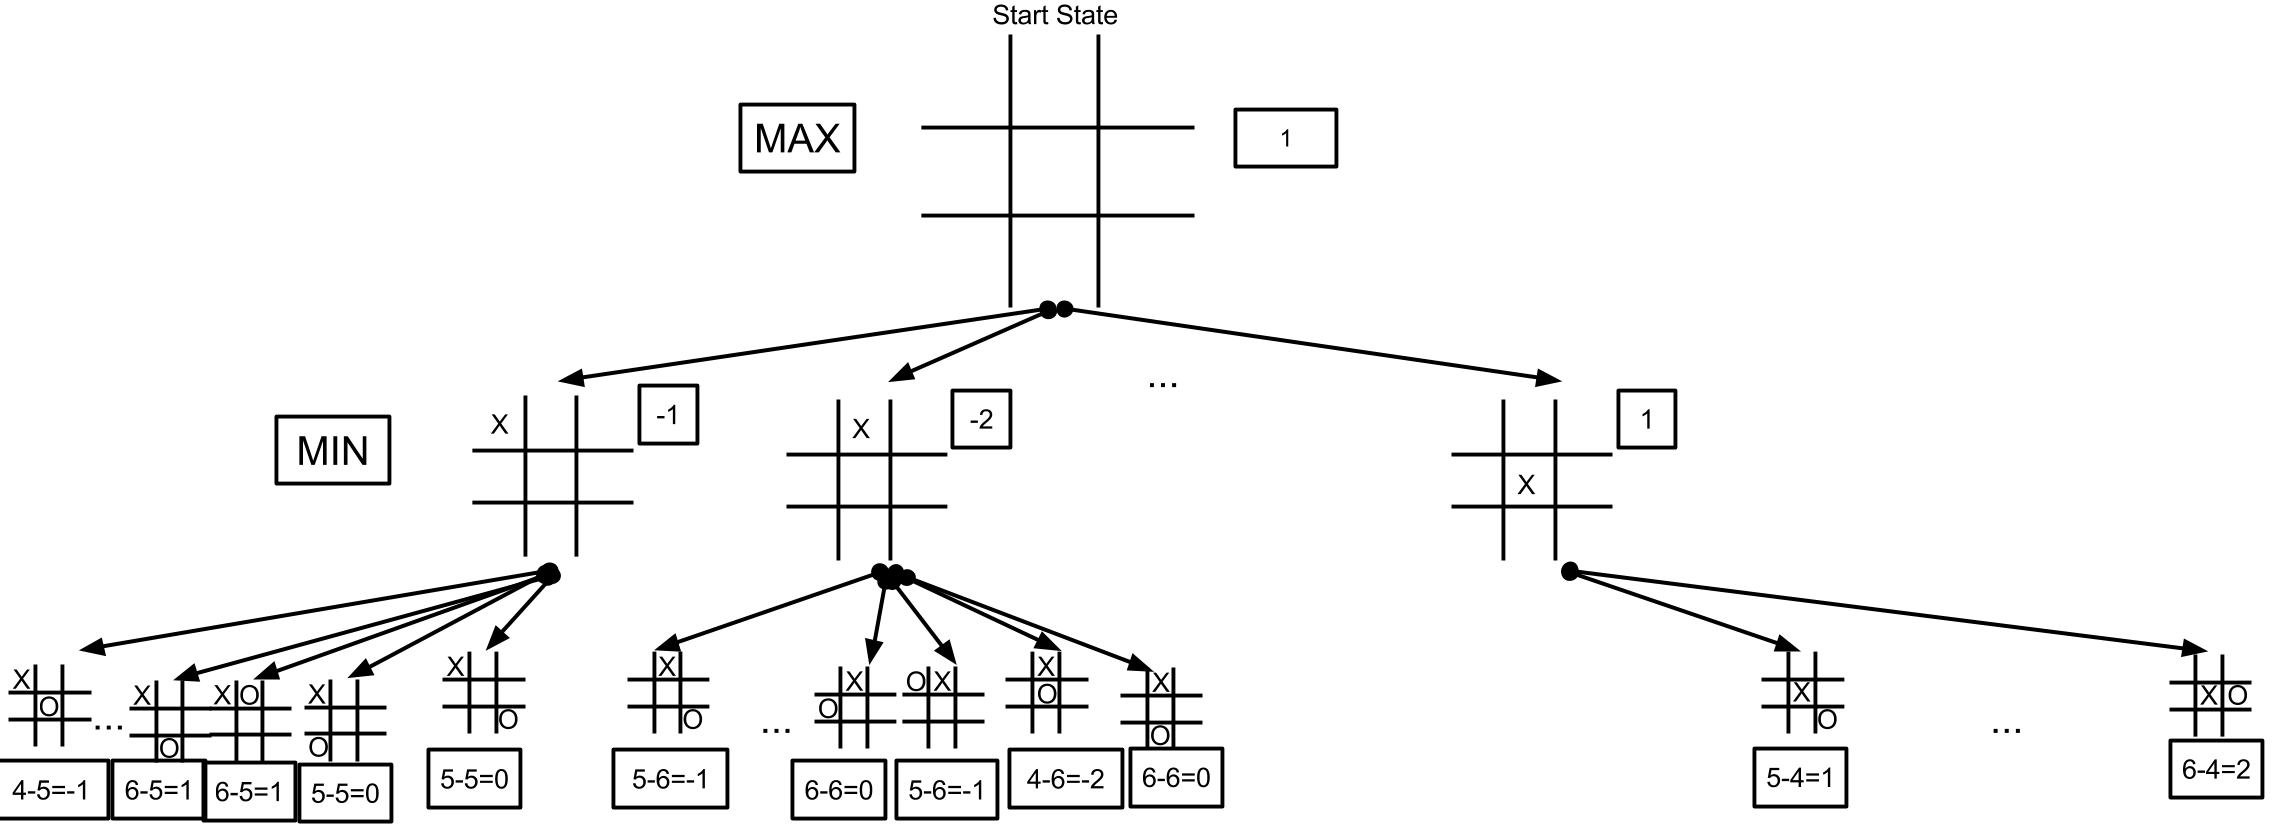
\includegraphics[scale=0.2]{figures/Minimax_Solved_TicTacToe_SearchTree_Template.png}
    \caption{Tic-Tac-Toe Minimax Search Tree}
    \label{fig:minimax_tree}
\end{figure}


\subsection{Alpha-Beta Pruning} (15pts) Show the upper and lower bounds for each node that are found using alpha-beta pruning. Show which nodes in the tree will be pruned. Explain why pruning depends on the node ordering. You can use the \texttt{TicTacToe-AlphaBetaTree-Template} provided at~\href{https://docs.google.com/drawings/d/1Uafusj47EC6_wIXe2KCkn_wBORsNegwYwHa6j_A3gBQ/edit?usp=sharing}{\color{blue}{HWs Public/HW2}}; make a copy and move the copy to your own Google Drive to edit it.\\
\\
See Figure~\ref{fig:alphabeta_tree}.
\begin{figure}[h]
    \centering
    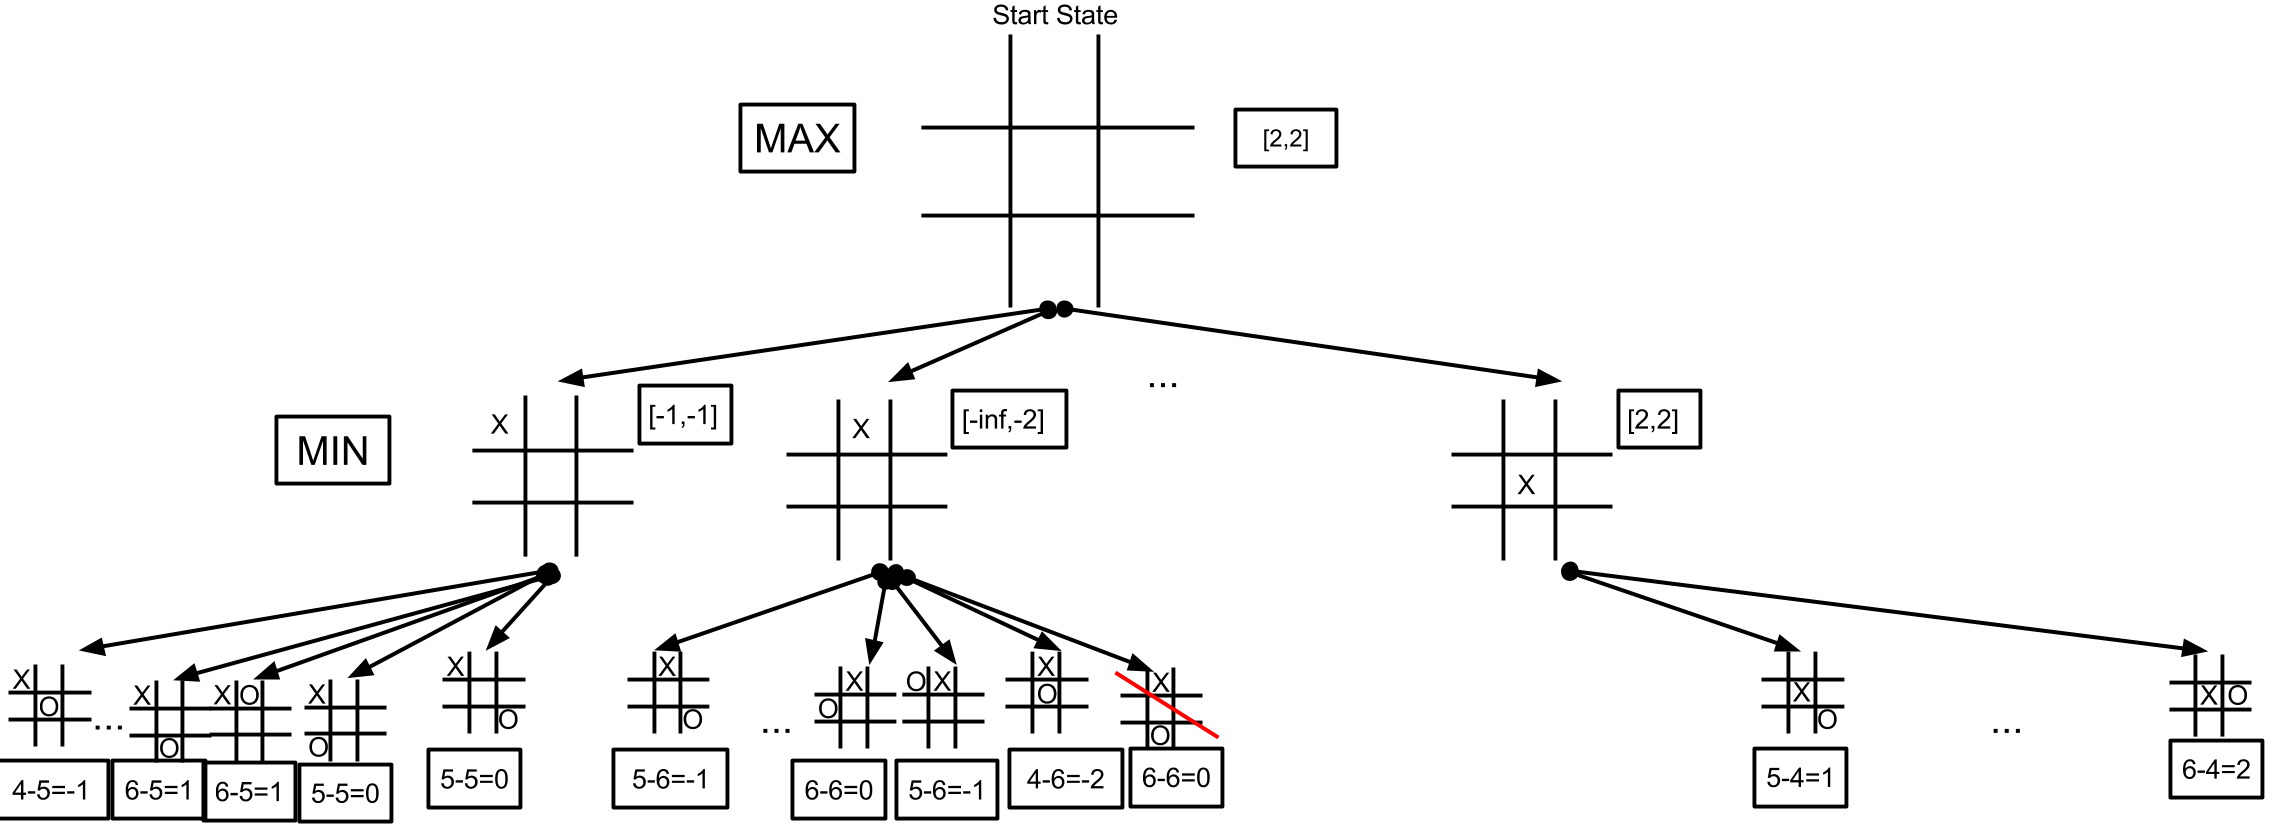
\includegraphics[scale=0.2]{figures/AB_Solved_TicTacToe_SearchTree_Template.png}
    \caption{Tic-Tac-Toe AlphaBeta Search Tree}
    \label{fig:alphabeta_tree}
\end{figure}

Pruning occurs when there is enough information gathered by traversing leaves to be certain that for their respective parent min nodes, max will never select a certain min node. When this condition is reached, the following subtree of that same parent can be pruned.

Pruning depends on node ordering because the order of the subsequent min nodes beyond the set of leaves of the leftmost child node at depth 1 determines when the DFS for Alpha-Beta pruning can return from the current min node and begin to search through the next min node. The DFS traverses the tree from the left-most leaf child depth-wise to the rightmost child of that parent and so on. If in subsequent min nodes, there exists a node that has an upper bound of value less than the current min node that would be selected by max, then the entire following set of subtrees with the same parent can be pruned as max would never select a min node that has an upper bound of less than the current lowest min node. In the worst case, if these minimum values always occur at the rightmost children of their respective parents such that all neighbors left of these minimum values are greater than or equal to the current min node value and each (right-located) minimum value is greater than the minimum values for the preceding min nodes, then the entire tree will be searched and no pruning will occur at all.  \\

Using figure 2 as an example, if the leaf node of the second min node with value -2 occurred as the first left-most child of that min node, then the rest of the nodes of that parent would have been pruned as -2 is less than the value of the first min node (-1). Max would never choose a node with less value than the current minimum, satisfying the condition to prune the subsequent children and progressing to the third min-node.



\end{document}
